\documentclass[addpoints,12pt]{exam}
\usepackage{amsmath}
\usepackage{amsthm}
\usepackage{amsfonts}
\usepackage{systeme}
\usepackage{graphicx}
\usepackage{caption}
\usepackage{xfrac}
\usepackage{physics}
\usepackage{microtype}
\usepackage{eulervm}
%\usepackage[framemethod=tikz]{mdframed}
\usepackage{thmtools}
\usepackage{etoolbox}
%\usepackage{fouriernc}
\usepackage{mdframed}
\usepackage[overload]{empheq}
\usepackage{adjustbox}
\usepackage{enumitem}
\usepackage[explicit]{titlesec}
% adds in \varnothing for empty set
\usepackage{amssymb}
% adds in formated SI units
%\usepackage{siunitx}
\usepackage{pgfplots}

\pagestyle{headandfoot}
\runningfootrule
\firstpageheadrule
\runningheadrule

\newcommand{\class}{Math 0097}
\newcommand{\sem}{2211}
\newcommand{\due}{}
\newcommand{\sect}{4.1}
\newcommand{\topic}{Solving Systems of Linear Equations by Graphing}

\firstpageheader{\class}{\sect - \topic}{}
\runningheader{\class}{\sect - \topic}{}
\firstpagefooter{\class}{}{Page \thepage\ of \numpages}
\runningfooter{\class}{}{Page \thepage\ of \numpages}

\newif\ifprintselected
\printselectedtrue
%\printselectedfalse

\newenvironment{select}
{\ifprintselected
	\printanswers
	\fi
}
{}

\theoremstyle{definition}
\newtheorem{theorem}{Theorem}
%\newtheorem{example}{Example}[subsection]
%\newtheorem{definition}{Definition}
%\newmdtheoremenv{definition}{Definition}[subsection]
%\newmdtheoremenv{example}{Example}[subsection]
\AtBeginEnvironment{defn}{\begin{minipage}{\textwidth}}
\AtEndEnvironment{defn}{\end{minipage}}
%\AtBeginEnvironment{example}{\begin{minipage}{\textwidth}}
%\AtEndEnvironment{example}{\end{minipage}}
\newcommand{\iu}{{i\mkern1mu}}

\setlength{\gridsize}{5mm}
\setlength{\gridlinewidth}{0.1pt}

\printanswers
\DeclareMathSizes{12}{12}{12}{12}

%%%%%%%%%%%%%%%%%%%%%%%%
% Create bars around subsubsection
%%%%%%%%%%%%%%%%%%%%%%%%

\titleformat{\subsubsection}
   {\large\bfseries}% format
   {}% label
   {0pt}% sep
   {\titlerule \vspace{.1in} #1}% before code
      [{\titlerule[0.4pt]\vspace{.1in}}]% after code
\titlespacing{\subsubsection}
   {0pt}% left
   {0pt}% before sep
   {\baselineskip}% after sep
   
%%%%%%%%%%%%%%%%%%%%%%%
% Create line break after definition label
%%%%%%%%%%%%%%%%%%%%%%%   
\newtheoremstyle{break}
  {\topsep}{\topsep}%
  {}{}%\itshape
  {\bfseries}{}%
  {\newline}{}%
\theoremstyle{break}
\newmdtheoremenv{definition}{Definition}[subsection]
\theoremstyle{break}
\newtheorem{example}{Example}[subsection]

%%%%%%%%%%%%%%%%%%%%%%
% start document
% set section, subsection (use n-1 for sub)
%%%%%%%%%%%%%%%%%%%%%%


\begin{document}
\setcounter{section}{4}
\setcounter{subsection}{0}

\subsection{Solving Systems of Linear Equations by Graphing}

\vspace{.15in}

\begin{definition}[System of Equations]
\mbox{}\\
\vspace{-.5in}
\begin{itemize}
\item a group of two or more equations that are solved at the same time
\item the solution is a point where both equations intersect
\item the solution satisfies both equations
\end{itemize}
\end{definition}

\vspace{.15in}

\begin{example}
Determine which of the points below are a solution to the system:
\[\systeme{2x-3y=-4,2x+y=4}\]

\begin{enumerate}
\begin{minipage}{.5\textwidth}
\item $(1,2)$
\end{minipage}%
\begin{minipage}{.5\textwidth}
\item $(7,6)$
\end{minipage}%
\end{enumerate}
\end{example}

\vspace{2in}

\begin{mdframed}
\textbf{Methods for Solving Systems of Equations}
\begin{enumerate}
\item Graphing
\item Substitution
\item Elimination/Addition
\item CAS (Computer Algebra Software)
\end{enumerate}
\end{mdframed}

\newpage

\subsubsection*{Method: Graphing}

\vspace{.15in}
\begin{mdframed}
\begin{enumerate}
\item Graph both equations on the same plane.
\item Determine if and where the lines intersect.
\item Algebraically verify whether the point is a solution or not.
\end{enumerate}
\end{mdframed}

\vspace{.15in}

\begin{example}
Solve the system by graphing: 
\[\systeme{2x+y=6,2x-y=-2}\]
\begin{figure}[h]
\centering
\begin{tikzpicture}
\begin{axis}[
  width=0.7\linewidth,
  axis lines=middle,
  grid,
  ymin=-6,
  ymax=6,
  ytick={-5,...,5},
  yticklabels={,,},
  ylabel={y},
  xmin=-6,
  xmax=6,
  xtick={-5,...,5},
  xticklabels={,,},
  xlabel={x}]

\addplot[draw=none] coordinates {(1,1)};
\end{axis}
\end{tikzpicture}
\end{figure}
\end{example}

\newpage

\begin{example}
Solve the system by graphing: 
\[\systeme{y = -x + 6, y = 3x - 6}\]
\begin{figure}[h]
\centering
\begin{tikzpicture}
\begin{axis}[
  width=0.7\linewidth,
  axis lines=middle,
  grid,
  ymin=-6,
  ymax=6,
  ytick={-5,...,5},
  yticklabels={,,},
  ylabel={y},
  xmin=-6,
  xmax=6,
  xtick={-5,...,5},
  xticklabels={,,},
  xlabel={x}]

\addplot[draw=none] coordinates {(1,1)};
\end{axis}
\end{tikzpicture}
\end{figure}
\end{example}

\newpage

\subsubsection*{Other Types of Solutions}
\begin{figure}[h]
\centering
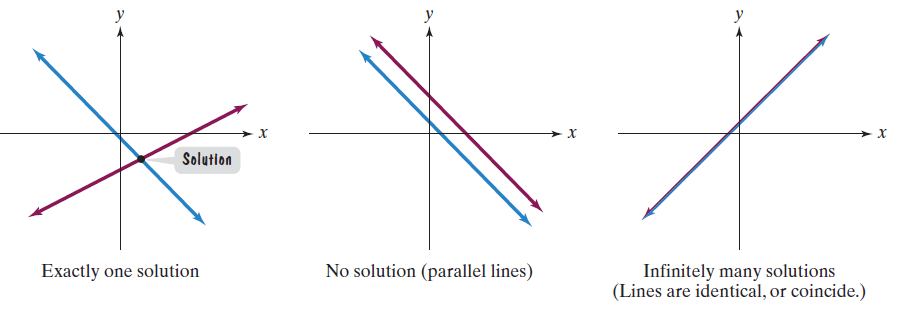
\includegraphics[scale=.6]{../images/types_of_systems_solutions}
\end{figure}
\vspace{.5in}

\begin{example}
Solve the system by graphing: 
\[\systeme{y = 3x - 2, y = 3x + 1}\]
\begin{figure}[h]
\centering
\begin{tikzpicture}
\begin{axis}[
  width=0.5\linewidth,
  axis lines=middle,
  grid,
  ymin=-6,
  ymax=6,
  ytick={-5,...,5},
  yticklabels={,,},
  ylabel={y},
  xmin=-6,
  xmax=6,
  xtick={-5,...,5},
  xticklabels={,,},
  xlabel={x}]

\addplot[draw=none] coordinates {(1,1)};
\end{axis}
\end{tikzpicture}
\end{figure}
\end{example}

\newpage

\begin{example}
Solve the system by graphing: 
\[\systeme{x+y = 3, 2x + 2y = 6}\]
\begin{figure}[h]
\centering
\begin{tikzpicture}
\begin{axis}[
  width=0.7\linewidth,
  axis lines=middle,
  grid,
  ymin=-6,
  ymax=6,
  ytick={-5,...,5},
  yticklabels={,,},
  ylabel={y},
  xmin=-6,
  xmax=6,
  xtick={-5,...,5},
  xticklabels={,,},
  xlabel={x}]

\addplot[draw=none] coordinates {(1,1)};
\end{axis}
\end{tikzpicture}
\end{figure}
\end{example}
\end{document}